\chapter{PERSEPSI GURU SEKOLAH DASAR TERHADAP SISTEM PENASEHAT PEMBELAJARAN BERDASARKAN KEMIRIPAN SISWA}

\section{Pendahuluan}
    Perkembangan teknologi pembelajaran memiliki dampak dan pengaruh yang signifikan terhadap proses pembelajaran siswa. Jepang, yang memiliki salah satu sistem pendidikan terbaik di dunia, mengembangkan berbagai infrastruktur digital pendukung. Jepang sering dijadikan acuan oleh negara-negara berkembang sebagai model untuk meningkatkan kualitas pendidikan \citep{Vicente2024}. Sistem pendidikan Indonesia masih banyak yang dapat dipelajari dari Jepang. Berbeda dengan Jepang, sistem pendidikan di Indonesia belum sepenuhnya menerapkan teknologi pembelajaran di semua sekolah sebagai alat untuk mendukung pembelajaran atau memantau siswa di sekolah.
    
    Salah satu platform teknologi pembelajaran yang dikembangkan di Jepang adalah MONSAKUN dari Universitas Hiroshima untuk anak-anak sekolah dasar \citep{Hirashima2014}. MONSAKUN adalah lingkungan pembelajaran berbasis komputer yang memfasilitasi pembelajaran melalui soal-soal matematika praktis yang melibatkan operasi penjumlahan dan pengurangan tunggal. MONSAKUN bertujuan untuk memberikan penilaian dan umpan balik otomatis atas ujian yang dikirimkan oleh siswa sekolah dasar. Hal ini memungkinkan guru untuk memantau kemajuan individu siswa dan kemajuan kelas secara keseluruhan secara real-time \citep{Hirashima2007}. MONSAKUN menghasilkan data log proses berpikir siswa sekolah dasar dalam belajar aritmatika dasar. Data Log ini kemudian dianalisis dalam \citep{Hasanah2015}.
    
    Dalam studi ini, kami mengembangkan teknik visualisasi menggunakan Self-Organizing Maps (SOM) Kohonen. SOM merupakan alat yang berharga untuk memahami dan menganalisis data berdimensi tinggi \cite{Budayan2009}. Dalam konteks pendidikan, visualisasi merupakan pendekatan intuitif bagi guru yang belum tentu familiar dengan ilmu data. Penelitian sebelumnya yang dilakukan oleh \citep{Tibyani2024,Tibyani2025} membahas tentang mengidentifikasi siswa dengan kinerja rendah dan memberikan bimbingan untuk meningkatkan prestasi akademik mereka melalui analisis data perilaku belajar. Menggunakan metode Self-Organizing Maps-m-Ary Tree (SOM-m-AT), karakteristik belajar siswa dipetakan ke dalam representasi topologis dua dimensi untuk membantu guru mengenali pola belajar mereka. Hasil menunjukkan bahwa siswa dengan perilaku belajar serupa cenderung berkelompok. Representasi dimensi rendah ini kemudian digunakan untuk mengidentifikasi siswa berprestasi rendah dan siswa lain yang memiliki karakteristik belajar serupa tetapi hasil yang lebih baik. Kesamaan belajar kemudian digunakan untuk menghasilkan saran bagi siswa dengan kinerja rendah tanpa harus mengubah pola belajar mereka secara drastis. Karakteristik utama sistem ini terletak pada kemampuannya untuk mengelompokkan siswa berdasarkan kesamaan topologis dalam perilaku belajar, tanpa memerlukan guru untuk memiliki pemahaman mendalam tentang teknik analisis data. Hal ini membuatnya sangat cocok untuk diterapkan di tingkat pendidikan dasar, di mana guru membutuhkan alat intuitif untuk memberikan bimbingan yang terarah.
    
    Untuk mengeksplorasi penerapan nyata pendekatan berbasis data ini dalam konteks pendidikan yang berbeda, penting untuk menganalisis bagaimana sistem semacam ini dipersepsikan oleh pengguna yang dituju—guru. Memahami penerimaan teknologi ini oleh guru sangat penting ketika sistem akan diimplementasikan di lingkungan dengan tingkat kesiapan teknologi yang berbeda dari tempat sistem tersebut dikembangkan. Oleh karena itu, studi ini berfokus pada penyelidikan persepsi guru matematika sekolah dasar di Kota Malang, Indonesia, menggunakan Model Penerimaan Teknologi (TAM) \cite{Anisa2021,Davis1989,Venkatesh2000} sebagai kerangka analitis.
    
    Bagian-bagian selanjutnya dari makalah ini disusun sebagai berikut: Bagian 2 memberikan gambaran singkat tentang metodologi penelitian dalam studi ini. Bagian 3 menyajikan hasil dan pembahasan, sementara Bagian 4 menyimpulkan makalah dan mengusulkan arah penelitian di masa depan.

\section{Metodologi Penelitian}

    Penelitian ini menggunakan pendekatan kuantitatif dengan melakukan survei, sehingga tidak melibatkan pembentukan hipotesis. Tujuan utama penelitian ini adalah untuk memahami pandangan guru tentang sistem bimbingan belajar di sekolah dasar. Pengumpulan data akan didasarkan pada fakta yang dirasakan oleh responden. 
    
    Teknik pengumpulan data kuesioner adalah metode yang digunakan untuk mengumpulkan informasi atau pendapat dari responden melalui serangkaian pertanyaan tertulis. Kuesioner biasanya terdiri dari berbagai jenis pertanyaan, seperti pilihan ganda, skala Likert, atau pertanyaan terbuka. Kuesioner adalah teknik pengumpulan data yang dilakukan dengan memberikan serangkaian pertanyaan atau pernyataan tertulis kepada responden untuk dijawab [10]. Kuesioner dibagi menjadi dua jenis: terbuka dan tertutup.
    
    Dalam penelitian ini, kuesioner yang digunakan adalah kuesioner tertutup, di mana jawaban sudah disediakan dan responden hanya perlu memilih respons mereka. Peneliti juga menggunakan skala Likert 4 poin (bilangan genap) untuk menghindari bias kecenderungan pusat, yang dapat terjadi pada skala Likert bilangan ganjil. Skala Likert ini mencakup empat opsi jawaban: sangat tidak setuju, tidak setuju, setuju, dan sangat setuju. Skala Likert digunakan untuk mengukur sikap, pendapat, dan persepsi individu atau kelompok terhadap fenomena sosial. Setiap pilihan jawaban diberi skor, dan responden harus menunjukkan apakah mereka mendukung pernyataan (positif) atau tidak mendukungnya (negatif) [10].
    
    Setelah peneliti menyiapkan elemen-elemen yang diperlukan untuk pengumpulan data, mereka mencari populasi yang akan digunakan sebagai sampel data. Sampel adalah bagian dari jumlah total dan karakteristik yang dimiliki oleh populasi \citep{Turner2020}. Populasi adalah keseluruhan elemen yang akan diteliti dan memiliki karakteristik yang sama \citep{Norman2024}. Populasi dapat terdiri dari individu dalam suatu kelompok, peristiwa, atau entitas lain yang sedang diteliti. Dalam studi ini, populasi yang ditargetkan terdiri dari guru sekolah dasar di Malang, di mana persepsi mereka digunakan sebagai data untuk penelitian ini. Peneliti melakukan studi dengan guru sekolah dasar sebagai populasi, berjumlah 20 orang. Berikut adalah jumlah peserta penelitian berdasarkan jumlah responden yang mengajar siswa sekolah dasar.

    \begin{figure}[H]
        \centering
        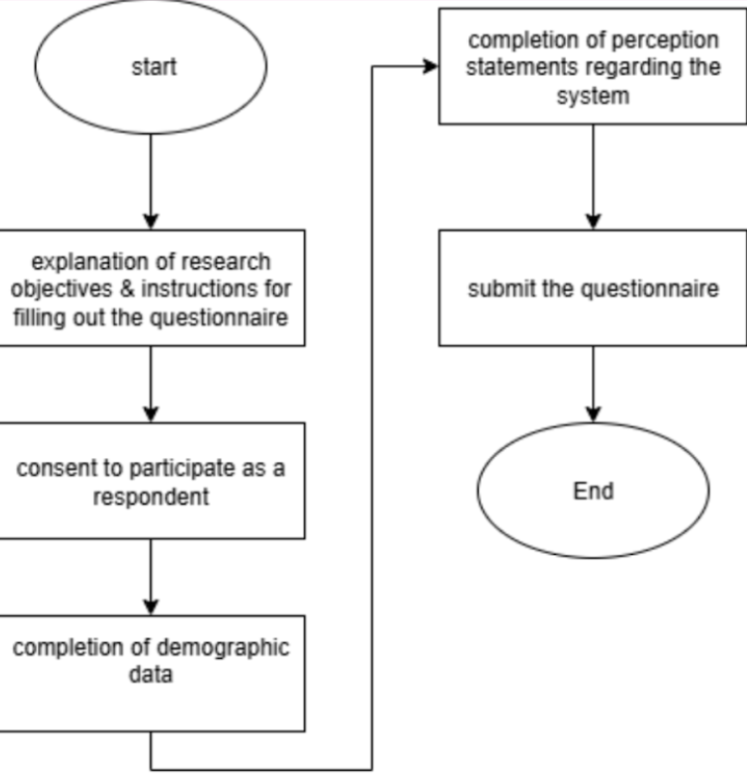
\includegraphics[width=0.7\textwidth]{Gambar/gambar7.2.png}
        \caption{Pengumpulan Data}
    \end{figure}

    Pada tahap penjelasan, peneliti menjelaskan cara mengisi kuesioner, termasuk pernyataan dan variabel yang terkandung di dalamnya. Kuesioner ini mencakup variabel yang mencerminkan persepsi responden terhadap sistem bimbingan belajar. Tahap berikutnya adalah persetujuan responden. Responden adalah guru sekolah dasar di Malang, dengan usia rata-rata 35 tahun, pengalaman kerja rata-rata 7 tahun, tingkat pendidikan tertinggi rata-rata sarjana (S1), dan sebagian besar di antaranya mengajar mata pelajaran matematika. Setelah itu, dilanjutkan dengan tahap pengisian pernyataan persepsi, diikuti dengan pengembalian kuesioner.Alasan mereka dipilih sebagai responden target dalam studi ini adalah karena mereka adalah guru matematika yang mengajar di sekolah dasar di Kota Malang.

\subsection{Model Penerimaan Teknologi (TAM)}

    Model Penerimaan Teknologi (TAM) adalah salah satu model teoritis yang dikembangkan untuk memahami dan memprediksi penerimaan teknologi oleh pengguna. Model ini pertama kali diperkenalkan oleh Fred D. Davis pada tahun 1986 sebagai adaptasi dari Teori Tindakan Berpikir (TRA) oleh Fishbein dan Ajzen.
    
    TAM menjelaskan bahwa dua faktor utama mempengaruhi penerimaan teknologi: Kegunaan yang Dirasakan (PU) dan Kemudahan Penggunaan yang Dirasakan (PEOU) [5]. Kegunaan yang Dirasakan merujuk pada sejauh mana seseorang percaya bahwa menggunakan sistem tertentu akan meningkatkan kinerjanya, sementara Kemudahan Penggunaan yang Dirasakan merujuk pada sejauh mana seseorang percaya bahwa menggunakan sistem tersebut akan bebas dari upaya yang signifikan.
    
    Model ini menekankan bahwa jika pengguna menganggap teknologi sebagai sesuatu yang berguna dan mudah digunakan, mereka lebih cenderung memiliki sikap positif terhadap penggunaannya, yang pada gilirannya akan mendorong niat dan keputusan mereka untuk menggunakan teknologi tersebut.

    \begin{figure}[H]
        \centering
        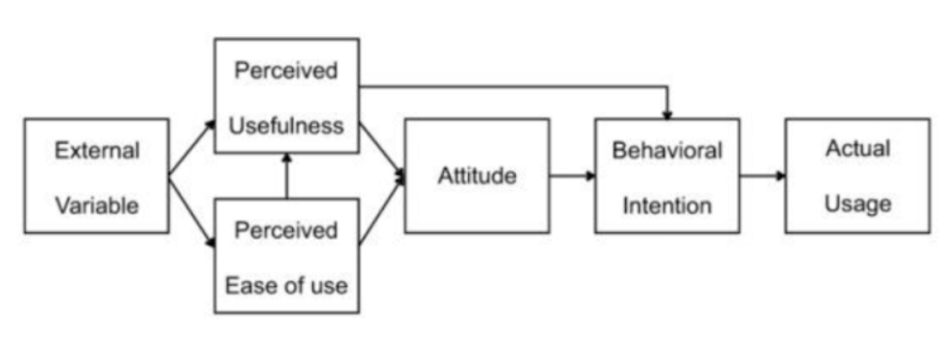
\includegraphics[width=0.7\textwidth]{Gambar/gambar7.3.png}
        \caption{Model Penerimaan Teknologi}
    \end{figure}

    Dalam Gambar 1, Model Penerimaan Teknologi (TAM) dapat diperluas melalui integrasi variabel eksternal, seperti dukungan organisasi, pelatihan, atau karakteristik individu, yang dapat mempengaruhi PU (Kegunaan yang Dirasakan) dan PEOU (Kemudahan Penggunaan yang Dirasakan) [6]. Hal ini membuat TAM relevan dalam berbagai konteks, termasuk bidang pendidikan.

    Di sisi lain, TAM banyak digunakan dalam konteks penelitian sistem informasi karena kesederhanaannya dan kemampuannya untuk menjelaskan niat perilaku terhadap penggunaan teknologi [6]. Dalam konteks pendidikan, model ini dapat digunakan untuk mengukur sejauh mana guru atau pendidik menerima dan bersedia menggunakan teknologi instruksional.

\subsection{Kontruksi TAM}

    Dalam adopsi teknologi baru di pendidikan, persepsi guru memainkan peran sentral. Oleh karena itu, untuk memahami faktor-faktor yang mempengaruhi penerimaan guru terhadap teknologi sistem penasihat, penelitian ini menggunakan pendekatan Model Penerimaan Teknologi (TAM) yang dikembangkan oleh Davis (1986) dan diperluas oleh Venkatesh dan Davis (2000).

    \begin{figure}[H]
        \centering
        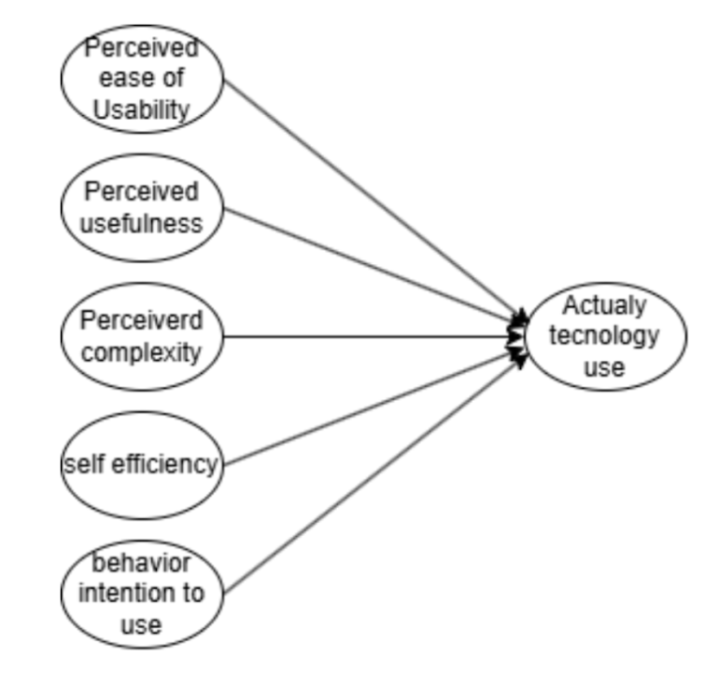
\includegraphics[width=0.7\textwidth]{Gambar/gambar7.4.png}
        \caption{Struktur Desain Penelitian Model}
    \end{figure}

    Model ini menjelaskan bahwa penerimaan teknologi dapat dipengaruhi oleh dua variabel utama: Kegunaan yang Dirasakan (PU) dan Kemudahan Penggunaan yang Dirasakan (PEOU). Selain itu, model ini juga dapat dikembangkan lebih lanjut dengan menambahkan variabel eksternal yang relevan dengan konteks penelitian, seperti Keyakinan Diri, Kompleksitas, Niat Perilaku untuk Menggunakan, dan Penggunaan Aktual. Model ini dapat dilihat pada Gambar 2.

    \begin{enumerate}
        \item Kemudahan Penggunaan yang Dirasakan
        
        Menjelaskan sejauh mana guru merasa bahwa sistem penasihat pembelajaran mudah dipelajari, dipahami, digunakan, dan diintegrasikan ke dalam aktivitas pengajaran.
        
        \item Kegunaan yang Dirasakan
        
        Menunjukkan keyakinan guru bahwa penggunaan sistem teknologi ini dapat meningkatkan efisiensi dan efektivitas dalam proses pengajaran dan pembelajaran, termasuk memberikan penilaian dan umpan balik kepada siswa.
        
        \item Kompleksitas yang Dirasakan
        
        Menilai tingkat kesulitan atau kompleksitas yang dirasakan oleh guru saat menggunakan sistem, baik dalam hal fitur, implementasi, maupun pemahaman terhadap hasil penilaian yang disediakan oleh sistem.
        
        \item Kepercayaan Diri
        
        Mengukur kepercayaan guru dalam mengoperasikan sistem, termasuk motivasi dan keterampilan mereka dalam menggunakan teknologi pendidikan dan memberikan umpan balik yang bermakna kepada siswa.
        
        \item Niat Perilaku untuk Menggunakan
        
        Menunjukkan sejauh mana guru memiliki niat atau keinginan untuk menggunakan sistem secara konsisten dalam kegiatan pengajaran, serta keterbukaan mereka untuk mengintegrasikan teknologi ke dalam proses pembelajaran.
        
        \item Penggunaan Teknologi yang Sebenarnya
        
        Mengacu pada tingkat penggunaan teknologi yang sebenarnya dalam aktivitas pembelajaran sehari-hari, termasuk sejauh mana guru menggunakan sistem untuk menilai, memantau, dan membimbing siswa.
    \end{enumerate}

\subsection{Analisis Data}

    Analisis data penelitian dilakukan menggunakan perangkat lunak IBM SPSS Statistics :

    \begin{enumerate}
        \item Uji Validitas
        
        Validitas berasal dari kata validitas, yang berarti sejauh mana alat ukur secara akurat dan tepat menjalankan fungsi pengukurannya [11]. Selain itu, validitas adalah ukuran yang menunjukkan apakah variabel yang diukur benar-benar mewakili variabel yang dimaksudkan untuk diteliti oleh peneliti [12].
        
        \item Uji Reliabilitas
        
        Keandalan adalah alat yang digunakan untuk mengukur kuesioner, yang berfungsi sebagai indikator variabel atau konstruk [13]. Sebuah kuesioner dikatakan andal atau dapat diandalkan jika respons seseorang terhadap pernyataan-pernyataan tersebut konsisten atau stabil dari waktu ke waktu. Keandalan suatu tes mengacu pada tingkat stabilitas, konsistensi, daya prediksi, dan akurasi.

        \item Analisis Data

        Analisis data adalah proses pencarian dan pengaturan data secara sistematis yang diperoleh dari wawancara, catatan lapangan, dan dokumentasi dengan mengelompokkan data ke dalam kategori, membaginya menjadi unit, mensintesisnya, mengaturnya ke dalam pola, memilih apa yang penting dan apa yang akan diteliti, serta menarik kesimpulan sehingga mudah dipahami oleh diri sendiri dan orang lain [10].

        \item Uji Normalitas

        Uji normalitas bertujuan untuk menentukan apakah residu atau variabel gangguan dalam model regresi mengikuti distribusi normal. Hal ini menunjukkan bahwa respons yang diberikan oleh responden dalam kuesioner akan bervariasi antara satu responden dengan responden lainnya. Oleh karena itu, uji normalitas dapat digunakan untuk menentukan apakah distribusi data pada pertanyaan tertentu memenuhi syarat normalitas. Uji normalitas sangat penting dalam statistik, terutama karena banyak metode analisis statistik mengasumsikan bahwa data yang digunakan berasal dari distribusi normal [14].

        \item Uji Multikolinearitas

        Multikolinearitas adalah fenomena dalam analisis regresi berganda yang terjadi ketika dua atau lebih variabel independen dalam model regresi memiliki hubungan linier yang sangat kuat. Hal ini menunjukkan adanya ketergantungan di antara variabel independen, yang dapat menyulitkan pemisahan efek individu masing-masing variabel terhadap variabel dependen. Keberadaan multikolinearitas dapat menyebabkan estimasi koefisien regresi yang tidak stabil dan tidak dapat diandalkan, serta meningkatkan varians koefisien regresi, yang dapat menyebabkan kesalahan saat menafsirkan hasil analisis [15].

        \item Uji Heteroskedastisitas

        Heteroskedastisitas adalah masalah yang terjadi dalam model regresi linier ketika varians kesalahan (residu) tidak konstan di seluruh nilai variabel independen. Dalam kehadiran heteroskedastisitas, varians residu cenderung berubah seiring dengan perubahan nilai variabel independen. Herbert Glejser mengembangkan uji baru untuk mendeteksi heteroskedastisitas. Uji ini melibatkan regresi nilai absolut residual dari model regresi asli terhadap variabel independen yang diduga terkait dengan varians residual. Jika koefisien regresi secara statistik signifikan, hal ini menunjukkan adanya heteroskedastisitas [16].

        \item Uji t

        Uji t adalah metode statistik yang digunakan untuk menentukan apakah ada perbedaan yang signifikan antara rata-rata dua kelompok data. Teknik ini sering digunakan dalam penelitian kuantitatif, terutama ketika peneliti ingin mengevaluasi efek atau perbedaan perlakuan antara dua kelompok yang dianalisis [17].

        \item Uji F

        Uji F dilakukan dengan membandingkan nilai F yang dihitung dari hasil regresi dengan nilai F tabel berdasarkan derajat kebebasan tertentu dan tingkat signifikansi yang telah ditentukan (biasanya 5\% atau 0,05) [18]. Jika nilai F yang dihitung lebih besar dari nilai F tabel, dapat disimpulkan bahwa semua variabel independen dalam model secara bersamaan memiliki efek signifikan terhadap variabel dependen.
    \end{enumerate}

\section{Hasil dan Pembahasan}

    Data dalam penelitian ini berasal dari skor kuesioner mengenai persepsi guru sekolah dasar di Malang terkait penggunaan sistem penasihat pembelajaran dalam konteks kelas. Penelitian ini dilakukan dengan pendekatan kuantitatif deskriptif melalui penyebaran kuesioner sebagai instrumen utama. Kuesioner yang terdiri dari 25 pertanyaan dibagikan kepada guru, dan wawancara juga dilakukan dengan guru yang mengajar di sekolah dasar. Jumlah responden dalam penelitian ini adalah 20 guru sekolah dasar.

\subsection{Uji Validitas}

    Uji validitas juga dilakukan menggunakan perangkat lunak IBM SPSS untuk mengukur hubungan antara skor setiap item dan skor total variabel pada instrumen penelitian. Tabel hasil uji validitas dapat dilihat pada tabel di bawah ini.

    \begin{table}[H]
        \centering
        \caption{Hasil Uji Validitas pada Variabel Kemudahan Penggunaan yang Dirasakan}
        \label{tab:uji-validitas-kemudahan}
        \begin{tabularx}{\textwidth}{p{4.5cm}lXXXl}
            \toprule
            \textbf{Variabel} & \textbf{Kode Item} & \textbf{Nilai Korelasi yang Dihitung} & \textbf{Nilai r-tabel} & \textbf{Sig.} & \textbf{Deskripsi} \\
            \midrule
            \multirow{4}{=}{Kemudahan Penggunaan yang Dirasakan}
                & X1.1 & 0.721 & 0.444 & 0.000 & Valid \\
                & X1.2 & 0.663 & 0.444 & 0.001 & Valid \\
                & X1.3 & 0.838 & 0.444 & 0.000 & Valid \\
                & X1.4 & 0.765 & 0.444 & 0.000 & Valid \\
            \bottomrule
        \end{tabularx}
    \end{table}

    Dalam Tabel 1, variabel diukur menggunakan empat item pernyataan (X1.1 hingga X1.4) yang bertujuan untuk menilai persepsi guru terhadap kemudahan pemahaman dan penggunaan sistem penasihat pembelajaran. Hasil uji menunjukkan bahwa semua item memiliki nilai korelasi di atas r-table (0.444) dan nilai signifikansi yang sangat rendah (p<0.01). Nilai korelasi berkisar antara 0.663 hingga 0.838, menunjukkan hubungan yang kuat dan signifikan antara setiap item dan skor total variabel.

    \begin{table}[H]
        \centering
        \caption{Hasil Uji Validitas pada Persepsi Kegunaan}
        \label{tab:uji-validitas-kegunaan}
        \begin{tabularx}{\textwidth}{p{4.5cm}lXXXl}
            \toprule
            \textbf{Variabel} & \textbf{Kode Item} & \textbf{Nilai Korelasi yang Dihitung} & \textbf{Nilai r-tabel} & \textbf{Sig.} & \textbf{Deskripsi} \\
            \midrule
            \multirow{5}{=}{Kegunaan yang Dirasakan}
                & X2.1 & 0.777 & 0.444 & 0.000 & Valid \\
                & X2.2 & 0.719 & 0.444 & 0.000 & Valid \\
                & X2.3 & 0.798 & 0.444 & 0.000 & Valid \\
                & X2.4 & 0.781 & 0.444 & 0.000 & Valid \\
                & X2.5 & 0.706 & 0.444 & 0.001 & Valid \\
            \bottomrule
        \end{tabularx}
    \end{table}

    Dalam Tabel 2, variabel diukur menggunakan lima item pernyataan (X2.1 hingga X2.5) yang dirancang untuk menangkap persepsi guru mengenai manfaat sistem dalam meningkatkan efektivitas pengajaran. Hasil analisis data menunjukkan bahwa semua item memiliki nilai r antara 0.706 dan 0.798, dengan signifikansi $\leq 0.001$, menunjukkan hubungan yang kuat dan signifikan.

    \begin{table}[H]     \centering
        \caption{Hasil Uji Validitas pada Kompleksitas}
        \label{tab:uji-validitas-kompleksitas}
        \begin{tabularx}{\textwidth}{p{4.5cm}lXXXl}
            \toprule
            \textbf{Variabel} & \textbf{Kode Item} & \textbf{Nilai Korelasi yang Dihitung} & \textbf{Nilai r-tabel} & \textbf{Sig.} & \textbf{Deskripsi} \\
            \midrule
            \multirow{3}{=}{Kompleksitas}
                & X3.1 & 0.869 & 0.444 & 0.000 & Valid \\
                & X3.2 & 0.865 & 0.444 & 0.000 & Valid \\
                & X3.3 & 0.617 & 0.444 & 0.004 & Valid \\
            \bottomrule
        \end{tabularx}
    \end{table}

    Dalam Tabel 3, variabel ini terdiri dari tiga item (X3.1 hingga X3.3) yang mengukur persepsi guru terhadap kompleksitas sistem. Meskipun konsepnya negatif, hasil korelasi menunjukkan bahwa semua item memiliki nilai r yang dihitung berkisar antara 0.617 hingga 0.869, menunjukkan korelasi yang kuat dan signifikan dengan skor total. Temuan ini mengonfirmasi bahwa item-item variabel dalam Kompleksitas secara efektif mengukur persepsi guru terhadap tantangan teknis atau kesulitan dalam menggunakan sistem. Nilai tertinggi, X3.1 (r = 0.869), menyoroti bahwa guru memberikan penekanan yang signifikan pada aspek teknis.

    \begin{table}[H]
        \centering
        \caption{Hasil Uji Validitas pada Self-Efficacy (Efektivitas Diri)}
        \label{tab:uji-validitas-self-efficacy}
        \begin{tabularx}{\textwidth}{p{4.5cm}lXXXl}
            \toprule
            \textbf{Variabel} & \textbf{Kode Item} & \textbf{Nilai Korelasi yang Dihitung} & \textbf{Nilai r-tabel} & \textbf{Sig.} & \textbf{Deskripsi} \\
            \midrule
            \multirow{5}{=}{Efektivitas Diri}
                & X4.1 & 0.811 & 0.444 & 0.000 & Valid \\
                & X4.2 & 0.782 & 0.444 & 0.000 & Valid \\
                & X4.3 & 0.658 & 0.444 & 0.002 & Valid \\
                & X4.4 & 0.651 & 0.444 & 0.002 & Valid \\
                & X4.5 & 0.452 & 0.444 & 0.045 & Valid \\
            \bottomrule
        \end{tabularx}
    \end{table}

    Dalam Tabel 4, variabel Self-Efficacy mencerminkan keyakinan guru dalam menggunakan sistem dan diukur melalui lima item (X4.1 hingga X4.5). Hasil uji validitas menunjukkan bahwa semua item valid, dengan nilai r berkisar antara 0.452 hingga 0.811, dan semua nilai signifikansi < 0.05. Meskipun satu item (X4.5) memiliki nilai korelasi mendekati ambang batas minimum (r = 0.452), nilainya tetap berada dalam rentang statistik yang dapat diterima. Hasil ini menunjukkan bahwa guru memiliki persepsi yang relatif konsisten tentang kemampuan mereka dalam mengoperasikan sistem pembelajaran, dan semua item instrumen valid dalam mengukur Self-Efficacy ini.

    \begin{table}[H]
        \centering
        \caption{Hasil Uji Validitas pada Niat Perilaku untuk Menggunakan}
        \label{tab:uji-validitas-niat-perilaku}
        \begin{tabularx}{\textwidth}{p{5cm}lXXXl}
            \toprule
            \textbf{Variabel} & \textbf{Kode Item} & \textbf{Nilai Korelasi yang Dihitung} & \textbf{Nilai r-tabel} & \textbf{Sig.} & \textbf{Deskripsi} \\
            \midrule
            \multirow{4}{=}{Niat Perilaku untuk Menggunakan}
                & X5.1 & 0.774 & 0.444 & 0.000 & Valid \\
                & X5.2 & 0.645 & 0.444 & 0.002 & Valid \\
                & X5.3 & 0.591 & 0.444 & 0.006 & Valid \\
                & X5.4 & 0.866 & 0.444 & 0.002 & Valid \\
            \bottomrule
        \end{tabularx}
    \end{table}

    Dalam Tabel 5, variabel ini mengukur niat dan kesediaan guru untuk menggunakan sistem secara berkelanjutan, yang dievaluasi melalui empat item pernyataan (X5.1 hingga X5.4). Hasil analisis menunjukkan bahwa semua item memiliki korelasi yang kuat dan signifikan dengan skor total, dengan nilai r berkisar antara 0.591 hingga 0.866. Nilai signifikansi untuk semua item berada di bawah 0.05, dengan sebagian besar di bawah 0.01, menunjukkan kekuatan pengukuran yang sangat baik. Hal ini menunjukkan bahwa guru menunjukkan tingkat konsistensi yang tinggi dalam respons mereka terkait niat untuk terus menggunakan sistem.

    \begin{table}[H]
        \centering
        \caption{Hasil Uji Validitas pada Penggunaan Teknologi Aktual}
        \label{tab:uji-validitas-penggunaan-teknologi}
        \begin{tabularx}{\textwidth}{p{5cm}lXXXl}
            \toprule
            \textbf{Variabel} & \textbf{Kode Item} & \textbf{Nilai Korelasi yang Dihitung} & \textbf{Nilai r-tabel} & \textbf{Sig.} & \textbf{Deskripsi} \\
            \midrule
            \multirow{4}{=}{Penggunaan Teknologi Aktual}
                & Y1.1 & 0.626 & 0.444 & 0.003 & Valid \\
                & Y1.2 & 0.830 & 0.444 & 0.000 & Valid \\
                & Y1.3 & 0.745 & 0.444 & 0.000 & Valid \\
                & Y1.4 & 0.626 & 0.444 & 0.003 & Valid \\
            \bottomrule
        \end{tabularx}
    \end{table}

    Dalam Tabel 6, variabel Penggunaan Teknologi Aktual mengukur sejauh mana guru menggunakan sistem penasihat pembelajaran dalam praktik pengajaran sehari-hari mereka. Variabel ini dievaluasi melalui empat item pernyataan (Y1 hingga Y4). Hasil uji validitas menggunakan korelasi Pearson menunjukkan bahwa tiga dari empat item memiliki nilai r lebih besar dari 0,444 dan nilai signifikansi kurang dari 0,05, menunjukkan validitas. Meskipun korelasi antara beberapa item dalam indikator yang sama bervariasi, hubungan antara setiap item dan skor total variabel Penggunaan Teknologi Aktual menunjukkan kekuatan korelasi yang tinggi dan signifikan. Semua item memiliki nilai korelasi jauh di atas ambang batas minimum 0.444 dan nilai signifikansi yang sangat rendah, menunjukkan bahwa setiap pernyataan dalam konstruksi Penggunaan Teknologi Aktual memenuhi kriteria validitas.


\subsection{Uji Reliabilitas}

    Uji reliabilitas dilakukan menggunakan metode Cronbach’s Alpha. Tujuan uji reliabilitas adalah untuk menentukan sejauh mana instrumen konsisten dan stabil dalam mengukur suatu konstruk. Uji reliabilitas dilakukan dengan bantuan perangkat lunak IBM SPSS untuk menilai konsistensi setiap item pada instrumen penelitian.

    \begin{table}[H]
        \centering
        \caption{Hasil Uji Reliabilitas Persepsi Guru Sekolah Dasar di Malang}
        \label{tab:uji-reliabilitas-guru}
        \begin{tabularx}{\textwidth}{p{6cm}ccl}
            \toprule
            \textbf{Variabel} & \textbf{Jumlah Item} & \textbf{Cronbach’s Alpha} & \textbf{Kesimpulan} \\
            \midrule
            Kemudahan Penggunaan yang Dirasakan & 4 & 0.724 & Terpercaya (Baik) \\
            Kegunaan yang Dirasakan              & 5 & 0.807 & Terpercaya (Baik) \\
            Kompleksitas                         & 3 & 0.701 & Terpercaya (Baik) \\
            Kepercayaan Diri                     & 5 & 0.730 & Terpercaya (Baik) \\
            Niat Perilaku untuk Menggunakan      & 4 & 0.679 & Terpercaya (Baik) \\
            Penggunaan Teknologi yang Sebenarnya & 4 & 0.626 & Terpercaya (Baik) \\
            \bottomrule
        \end{tabularx}
    \end{table}

    Dalam Tabel 7, hasil uji menunjukkan bahwa semua variabel dalam studi ini memiliki nilai Cronbach’s Alpha lebih dari 0,60, menunjukkan bahwa instrumen yang digunakan dapat diandalkan dan sesuai untuk analisis lebih lanjut.
    
\subsection{Analisis Data}

    \begin{table}[H]
        \centering
        \caption{Hasil Analisis Data Persepsi Guru Sekolah Dasar di Malang}
        \label{tab:analisis-data-guru}
        \begin{tabularx}{\textwidth}{p{6cm}ccccc}
            \toprule
            \textbf{Variabel} & \textbf{N} & \textbf{Min} & \textbf{Maks} & \textbf{Rata-rata} & \textbf{Simpangan Baku} \\
            \midrule
            Kemudahan Penggunaan yang Dirasakan & 20 & 10 & 16 & 12.50 & 1.469 \\
            Kegunaan yang Dirasakan              & 20 & 11 & 19 & 15.30 & 2.029 \\
            Kompleksitas                         & 20 & 4  & 8  & 6.00  & 1.451 \\
            Kepercayaan Diri                     & 20 & 9  & 15 & 12.60 & 1.353 \\
            Niat Perilaku untuk Menggunakan      & 20 & 9  & 15 & 12.40 & 1.501 \\
            Penggunaan Teknologi yang Sebenarnya & 20 & 10 & 15 & 12.00 & 1.376 \\
            \bottomrule
        \end{tabularx}
    \end{table}

    Berdasarkan analisis deskriptif pada Tabel 8, dapat dilihat bahwa secara umum, guru memiliki pandangan positif terhadap sistem penasihat pembelajaran digital. Skor rata-rata untuk Kemudahan Penggunaan yang Dirasakan adalah 12,50, menunjukkan bahwa guru merasa sistem tersebut cukup mudah digunakan. Skor tertinggi terdapat pada Kegunaan yang Dirasakan, dengan rata-rata 15,30, artinya guru menganggap sistem tersebut sangat bermanfaat. Sementara itu, Kompleksitas memiliki skor rata-rata 6,00, menunjukkan bahwa sistem terasa agak kompleks tetapi masih dapat dikelola. Skor rata-rata untuk Kepercayaan Diri adalah 12,60, menunjukkan bahwa guru merasa percaya diri dalam menggunakan sistem. Niat Perilaku untuk Menggunakan memiliki skor rata-rata 12,40, menunjukkan bahwa guru berniat untuk terus menggunakan sistem. Akhirnya, Penggunaan Teknologi Aktual memiliki skor rata-rata 12,00, yang menunjukkan bahwa guru telah menggunakan sistem tersebut secara sering. Secara keseluruhan, data menunjukkan bahwa guru menerima sistem tersebut dengan baik dan mendukung penggunaannya dalam proses pembelajaran.

\subsection{Uji Normalitas}

    \begin{table}[H]
        \centering
        \caption{Hasil Uji Normalitas Persepsi Guru Sekolah Dasar di Malang}
        \label{tab:uji-normalitas-guru}
        \begin{tabularx}{0.8\textwidth}{p{7cm}r}
            \toprule
            \textbf{Statistik} & \textbf{Nilai} \\
            \midrule
            N & 20 \\
            Rata-rata & 0.0000000 \\
            Simpangan baku & 0.74985014 \\
            Perbedaan Ekstrem Terbesar (Absolut) & 0.106 \\
            Perbedaan Ekstrem Terbesar (Positif) & 0.106 \\
            Perbedaan Ekstrem Terbesar (Negatif) & -0.084 \\
            Kolmogorov-Smirnov Z & 0.106 \\
            Signifikansi Asimtotik (dua ekor) & 0.200 \\
            \bottomrule
        \end{tabularx}
    \end{table}

    Berdasarkan Tabel 9, hasil uji menunjukkan bahwa nilai Asymp. Sig. adalah 0.200, yang lebih besar dari 0.05. Hal ini menunjukkan bahwa data residu dalam model regresi mengikuti distribusi normal. Oleh karena itu, salah satu persyaratan asumsi klasik dalam regresi linier, yaitu asumsi normalitas residu, telah terpenuhi. Selain itu, nilai perbedaan absolut ekstrem terbesar sebesar 0,106 menunjukkan bahwa tidak ada penyimpangan yang signifikan antara distribusi data residu dan distribusi normal teoretis. Berdasarkan hasil uji, nilai Asymp. Sig. sebesar 0,200, yang lebih besar dari 0,05. Hal ini menunjukkan bahwa data residu dalam model regresi mengikuti distribusi normal. Oleh karena itu, salah satu persyaratan asumsi klasik dalam regresi linier, yaitu asumsi normalitas residu, telah terpenuhi. Selain itu, nilai perbedaan absolut ekstrem sebesar 0,106 menunjukkan bahwa tidak ada penyimpangan yang signifikan antara distribusi data residu dan distribusi normal teoretis.

\subsection{Uji Multikolinearitas}

    \begin{table}[H]
        \centering
        \caption{Hasil Uji Multikolinearitas Persepsi Guru Sekolah Dasar di Malang}
        \label{tab:uji-multikolinearitas-guru}
        \begin{tabularx}{0.8\textwidth}{p{7cm}r}
            \toprule
            \textbf{Statistik} & \textbf{Nilai} \\
            \midrule
            N & 20 \\
            Rata-rata & 0.0000000 \\
            Simpangan baku & 0.74985014 \\
            Perbedaan Ekstrem Terbesar (Absolut) & 0.106 \\
            Perbedaan Ekstrem Terbesar (Positif) & 0.106 \\
            Perbedaan Ekstrem Terbesar (Negatif) & -0.084 \\
            Kolmogorov-Smirnov Z & 0.106 \\
            Signifikansi Asimtotik (dua ekor) & 0.200 \\
            \bottomrule
        \end{tabularx}
    \end{table}

    Berdasarkan Tabel 10, hasil uji multikolinearitas di atas menunjukkan bahwa semua variabel independen memiliki nilai Toleransi > 0,10 dan nilai VIF < 10. Nilai VIF tertinggi ditemukan pada variabel Niat Perilaku, yaitu 3.964, namun nilai ini masih jauh di bawah ambang batas kritis 10. Demikian pula, nilai Toleransi untuk semua variabel berada di atas 0.10, menunjukkan bahwa tidak ada indikasi serius multikolinearitas dalam model regresi. 

\subsection{Uji Heteroskedastisitas}

    \begin{table}[H]
        \centering
        \caption{Hasil Uji Heteroskedastisitas Persepsi Guru Sekolah Dasar di Malang}
        \label{tab:uji-heteroskedastisitas}
        \begin{tabularx}{\textwidth}{lcccc}
            \toprule
            \textbf{Variabel Independen} & \textbf{B} & \textbf{Std. Error} & \textbf{t} & \textbf{Sig.} \\
            \midrule
            (Konstanta) & -3.166 & 0.968 & -3.286 & 0.006 \\
            Kemudahan Penggunaan yang Dirasakan & 0.081 & 0.091 & 0.885 & 0.391 \\
            Persepsi Kegunaan & 0.107 & 0.066 & 1.623 & 0.127 \\
            Kompleksitas & 0.063 & 0.058 & 1.076 & 0.300 \\
            Kepercayaan Diri & 0.146 & 0.106 & 1.374 & 0.191 \\
            Niat Perilaku & -0.089 & 0.097 & -0.922 & 0.372 \\
            \bottomrule
        \end{tabularx}
    \end{table}

    Berdasarkan Tabel 11, hasil uji heteroskedastisitas menggunakan metode Glejser menunjukkan bahwa semua variabel independen memiliki nilai signifikansi lebih besar dari 0.05. Oleh karena itu, tidak ada variabel prediktor yang secara signifikan mempengaruhi nilai absolut residu. Berdasarkan hasil uji heteroskedastisitas menggunakan metode Glejser, semua variabel independen memiliki nilai signifikansi lebih besar dari 0.05. Oleh karena itu, tidak ada variabel prediktor yang secara signifikan mempengaruhi nilai absolut residu. Berdasarkan hasil uji heteroskedastisitas menggunakan metode Glejser, semua variabel independen memiliki nilai signifikansi lebih besar dari 0,05. Oleh karena itu, tidak ada variabel prediktor yang secara signifikan mempengaruhi nilai absolut residu.

\subsection{Uji t}

    \begin{table}[H]
        \centering
        \caption{Hasil Uji t Persepsi Guru Sekolah Dasar di Malang}
        \label{tab:uji-t}
        \begin{tabularx}{\textwidth}{lccccc}
            \toprule
            \textbf{Variabel Independen} & \textbf{B} & \textbf{Kesalahan Standar} & \textbf{Beta} & \textbf{t} & \textbf{Sig.} \\
            \midrule
            Konstanta & 7.330 & 2.659 & - & 2.757 & 0.015 \\
            Kemudahan Penggunaan yang Dirasakan & 0.199 & 0.251 & 0.212 & 0.792 & 0.442 \\
            Kegunaan yang Dirasakan & -0.288 & 0.181 & -0.425 & -1.594 & 0.133 \\
            Kompleksitas & -0.367 & 0.160 & -0.387 & -2.301 & 0.037 \\
            Keyakinan Diri & 0.207 & 0.291 & 0.203 & 0.711 & 0.489 \\
            Niat Perilaku & 0.499 & 0.266 & 0.544 & 1.878 & 0.081 \\
            \bottomrule
        \end{tabularx}
    \end{table}

    Berdasarkan hasil uji t parsial pada Tabel 12, hanya variabel Kompleksitas yang ditemukan memiliki pengaruh signifikan terhadap Penggunaan Teknologi Aktual, dengan nilai signifikansi (p) sebesar 0,037 < 0,05. Hal ini menunjukkan bahwa semakin kompleks sistem yang dirasakan oleh guru, semakin rendah kecenderungan mereka untuk benar-benar menggunakannya. Variabel lain seperti Kemudahan Penggunaan yang Dirasakan, Kegunaan yang Dirasakan, Keyakinan Diri, dan Niat Perilaku untuk Menggunakan tidak menunjukkan efek yang signifikan secara statistik, meskipun niat untuk menggunakan mendekati ambang batas signifikansi, menunjukkan potensi pengaruh yang memerlukan penyelidikan lebih lanjut dengan ukuran sampel yang lebih besar.

\subsection{Uji f}

    \begin{table}[H]
        \centering
        \caption{Hasil Uji F Persepsi Guru Sekolah Dasar di Malang}
        \label{tab:uji-f}
        \begin{tabularx}{\textwidth}{lccccc}
            \toprule
            \textbf{Sumber Variasi} & \textbf{Jumlah Kuadrat} & \textbf{df} & \textbf{Rata-rata Kuadrat} & \textbf{F} & \textbf{Sig.} \\
            \midrule
            Regresi & 25,317 & 5 & 5,063 & 6,635 & 0,002 \\
            Sisa & 10,683 & 14 & 0,763 & - & - \\
            Total & 36,000 & 19 & - & - & - \\
            \bottomrule
        \end{tabularx}
    \end{table}

    Berdasarkan hasil uji F pada Tabel 13, nilai F yang dihitung adalah 6,635 dengan tingkat signifikansi (p = 0,002). Nilai p sebesar 0,002 menunjukkan bahwa probabilitas terjadinya hasil ini secara kebetulan sangat kecil jika semua koefisien sebenarnya tidak memiliki pengaruh. Selain itu, nilai ini jauh lebih kecil daripada tingkat signifikansi 0,05, yang berarti model regresi secara keseluruhan secara statistik signifikan. Temuan ini mengonfirmasi bahwa persepsi guru terhadap berbagai atribut sistem secara signifikan berkontribusi dalam menjelaskan penggunaan sistem penasihat pembelajaran berbasis teknologi. Hasil ini juga memperkuat validitas model regresi yang digunakan, memberikan dasar statistik yang kokoh bahwa semua konstruk dalam kerangka kerja berperan dalam membentuk sikap dan perilaku guru terhadap penggunaan teknologi dalam pendidikan.

\section{Kesimpulan}

    Berdasarkan hasil analisis data dan pembahasan, penelitian ini menyimpulkan bahwa guru sekolah dasar di Kota Malang secara umum memiliki persepsi positif terhadap sistem penasihat pembelajaran digital dan terbuka terhadap implementasinya dalam kegiatan pembelajaran di kelas. Hal ini didukung oleh analisis deskriptif, yang menunjukkan nilai rata-rata yang relatif tinggi pada variabel utama TAM, seperti Kegunaan yang Dirasakan (rata-rata = 15,30) dan Kepercayaan Diri (rata-rata = 12,60), menunjukkan bahwa guru menganggap sistem ini bermanfaat dan merasa percaya diri dalam menggunakannya. Berdasarkan hasil uji t parsial (Tabel 12), dari lima variabel independen, hanya Kompleksitas yang memiliki pengaruh signifikan terhadap Penggunaan Teknologi Aktual (p = 0,037) dengan koefisien negatif (B = –0,367), artinya semakin kompleks sistem tersebut dipersepsikan oleh guru, semakin kecil kemungkinan mereka untuk menggunakannya. Variabel lain seperti Kemudahan Penggunaan yang Dirasakan (p = 0,442), Kegunaan yang Dirasakan (p = 0,133), Keyakinan Diri (p = 0,489), dan Niat Perilaku untuk Menggunakan (p = 0,081) tidak menunjukkan efek yang signifikan secara statistik, meskipun niat menunjukkan kecenderungan mendekati signifikansi. Selain itu, hasil uji F (Tabel 13) menunjukkan bahwa model regresi secara keseluruhan secara statistik signifikan, dengan nilai F sebesar 6.635 dan tingkat signifikansi p = 0.002. Ini berarti semua variabel independen secara kolektif memiliki pengaruh signifikan terhadap Penggunaan Teknologi Aktual. Hasil ini memperkuat validitas model regresi dan menunjukkan bahwa variabel yang diukur berkontribusi dalam menjelaskan perilaku guru dalam mengadopsi teknologi. Kesimpulannya, meskipun tidak semua variabel secara individu menunjukkan pengaruh yang signifikan, kombinasi persepsi guru tentang kemudahan penggunaan, kegunaan, dan kepercayaan diri memainkan peran penting dalam mendorong penggunaan sistem yang sebenarnya. Temuan ini menyoroti pentingnya mengurangi kompleksitas sistem dan menyediakan pelatihan yang memadai untuk mendukung adopsi teknologi yang lebih luas. Studi ini memberikan landasan yang kuat untuk mengembangkan kebijakan pendidikan berbasis teknologi yang selaras dengan penerimaan guru dan realitas pembelajaran di kelas sekolah dasar Indonesia.